%-------------------------------------------------------------------------------
\section{Introduction}
%-------------------------------------------------------------------------------
\label{sec:intro}


%\begin{figure}
%  \centering
%  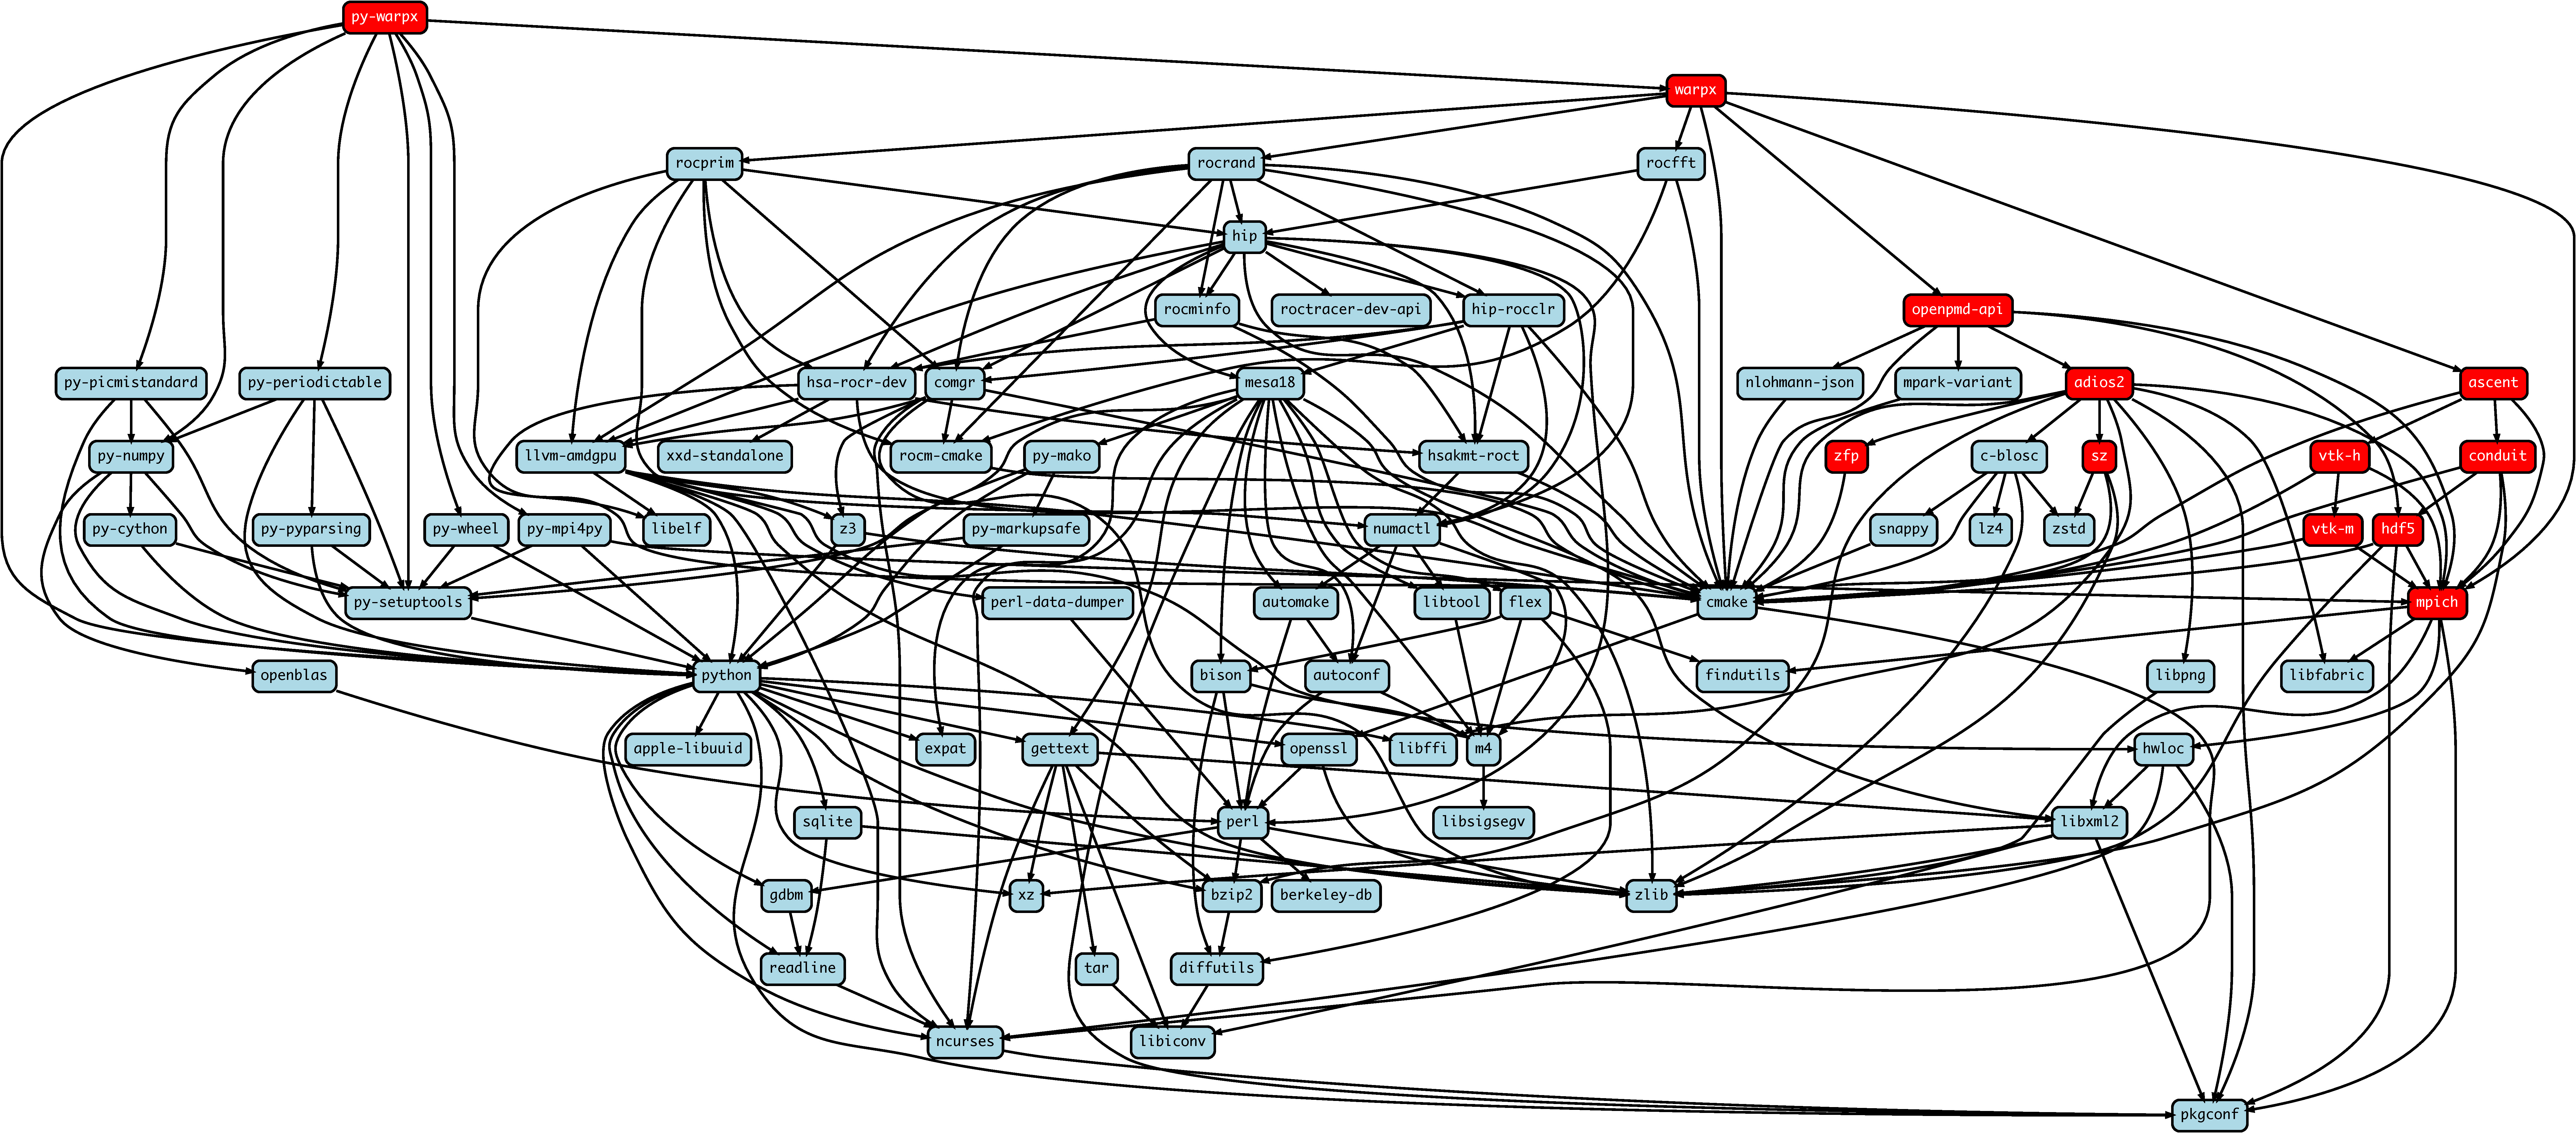
\includegraphics[width=.8\columnwidth]{figures/warpx.pdf}
%  \caption{ Dependencies of WarpX (built with AMD ROCm GPU support
%    enabled). E4S packages are shown in red.
%    \label{fig:warpx}
%  }
%\end{figure}

Managing dependencies for scientific software is notoriously
difficult~\cite{hoste+:pyhpc12,gamblin+:sc15,dubois2003johnny,hochstein+:2011-build}.
Scientific software is typically built from source to achieve good performance, and
configuring build systems, dependency versions, and compilers requires painstaking care.
In the past decade, the modularity of HPC software has increased due to well known
benefits such as separation of concerns, encapsulation, and code reuse. These enable
application codes to leverage fast math libraries~\cite{hypre,mfem,petsc,trilinos} and
GPU performance portability frameworks like RAJA~\cite{raja} and Kokkos~\cite{kokkos}.
However, the cost of modularity is integration complexity: consumers of components must
ensure that versions and other parameters are chosen correctly to ensure that all
integrated components work together.

{\it Package managers} emerged in the mid-1990's to mitigate the complexity of
integrating software packages in Linux distributions. In the past decade, their use has
exploded, particularly within language ecosystems like Python~\cite{pip},
Javascript~\cite{npm}, and Rust~\cite{cargo}, but also within the HPC community. The
HPC-centric package managers Spack~\cite{gamblin+:sc15} and
EasyBuild~\cite{hoste+:pyhpc12} are now widely used for software deployment at HPC
centers, and by developers and users installing their own software. The U.S. Exascale
Computing Project (ECP) has adopted Spack as the distribution tool for its
E4S~\cite{e4s} software stack (shown in Figure~\ref{fig:e4s-graph}), which contains
around 100 core software products and 500 required dependency packages.

\begin{figure*}
  \centering
  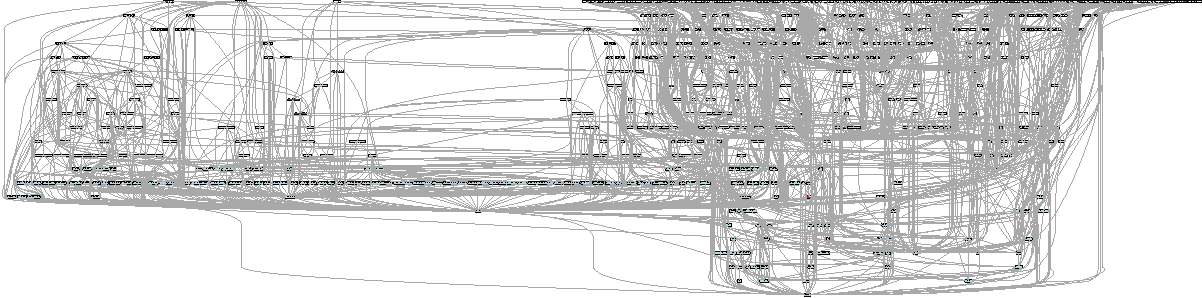
\includegraphics[width=\textwidth]{figures/e4s.pdf}
  \caption{
    Graph of package dependencies in the Extreme Scale Scientific Software Stack (E4S)~\cite{e4s}.
    Around 100 core software products are shown in red, and the 500 required dependencies
    are blue. The precise number of packages required for a deployment of E4S
    is system-specific, depending on platform and hardware (e.g., NVIDIA, AMD GPUs).
    \label{fig:e4s-graph}
  }
\end{figure*}

Package managers address the integration problem in two main ways. Systems like
EasyBuild and Nix~\cite{dolstra+:icfp08,dolstra+:lisa04} rely on human effort, where
maintainers develop fixed package configurations that define a common stack to be
shared among users. To deviate from the stack, users must update all configuration files
to ensure that versions and other parameters are consistent. More commonly, package
managers like Spack provide flexibility for the end user by incorporating {\it
  dependency solvers} at their core. Users can request arbitrary versions, and packages
declare {\it constraints} that bound the space of compatible configurations. The solver
selects a set of versions and configuration parameters that satisfy the user's
requirements and package constraints.

Dependency solving is NP-complete, even for a ``simple'' configuration space with only
packages and versions~\cite{dicosmo:edos,cox:version-sat}. Here, we focus on Spack's
dependency solver, known as the {\it concretizer}, which adds build options (variants),
compilers, target microarchitectures, and dependency versions to make the space even
larger. Most package managers use their own ad-hoc solver~\cite{abate2020dependency},
and Spack is no different; it has historically used its own {\it greedy} algorithm.
Heuristics were sufficient when there were only 245 packages~\cite{gamblin+:sc15}, but
now, Spack's mainline repository contains over 6,000 packages, each with many
constraints and options, and the original concretizer has begun to show its age. In
particular, it lacks:
\begin{itemize}
\item {\it Completeness}: in a growing number of cases, it may not find a solution even
  though one exists; and
\item {\it Optimality}: it provides no guarantees that it has found the ``best''
  of all valid solutions according to any criteria.
\end{itemize}

An increasing number of package managers use Boolean satisfiability (SAT) solvers to
resolve dependency constraints~\cite{abate2020dependency}, which works well for version
solving with a single optimization objective. With its added dimensions, Spack's solver
encodes a much larger configuration space {\it and} requires multi-objective
optimization. Encoding these semantics in pure SAT is {\it extremely} complex. Instead,
we have turned to Answer Set Programming
(ASP)~\cite{gebser+:asp-book,marek+:asp-origins}, a declarative model that allows us to
encode dependency semantics in a first-order, Prolog-like syntax. ASP solvers reduce
first-order logic programs to SAT and optimization, and they guarantee both complete
and optimal solutions. Unlike Prolog, they are also guaranteed to terminate. ASP
encodings are non-trivial, and this paper presents the first dependency solver capable
of making strong guarantees for the full generality of HPC dependency semantics.
Specifically, our contributions are:

\begin{enumerate}
\item A general mapping of Spack's DSL, compatibility semantics, and optimization rules
  to ASP;
\item A technique to optimize for reuse of existing builds in combinatorial package
  solves;
\item An ASP solver implementation in Spack that enables {\it complete} and {\it
  optimal} solutions; and
\item An evaluation of our system's performance on the E4S repository with tens of
  thousands of packages.
\end{enumerate}

Together, these contributions allow us to replace Spack's original concretizer with a
complete, optimizing solver, written in around 800 lines of declarative ASP. This
represents a leap forward in capability, maintainability, and extensibility to the
ever-increasing complexity of HPC software.
